\documentclass[10pt,twocolumn]{article}
\usepackage[margin=1in]{geometry}
\usepackage{booktabs}
\usepackage{amsmath}
\usepackage{graphicx}
\usepackage{hyperref}
\usepackage{xcolor}
\usepackage{cite}

\title{\textbf{EMMI: Edge Multi-Modal Intelligence via Match Fusion\\and Contrastive Autoencoding}}
\author{Motahareh Sohrabi}
\date{}

\begin{document}
\maketitle

% ============================================================
\section{Introduction}
% ============================================================

As edge systems become increasingly autonomous, their
effectiveness depends on the ability to reason across heterogeneous modalities under strict resource constraints. In
many operational environments, actionable insight emerges not
from a single source of information but from jointly interpreting visual observations, sensor measurements, telemetry,
and contextual data. This reliance on multi-modal reasoning
has created growing interest in intelligent systems capable of
integrating diverse information sources to support timely and
context-aware decision-making at the edge. Recent advances
in Multimodal Large Language Models (MLLMs) provide
a promising foundation for achieving such capabilities by
enabling unified processing of heterogeneous inputs.

Unlike conventional lightweight multi-modal models designed for specific tasks, MLLMs can capture higher-order
relationships among heterogeneous inputs and perform contextual cross-modal reasoning within a unified architecture. These
capabilities enable more flexible and generalizable decision-making across complex environments. However, achieving this
level of multi-modal intelligence requires large-scale models
with substantial computational, memory, and communication
requirements, creating a significant deployment gap between
the capabilities of modern MLLMs and the resources available
on edge platforms.

To enable MLLM capabilities on edge platforms, existing
deployment strategies have explored reducing model complexity, utilizing remote compute resources, and minimizing
communication costs. However, these approaches address individual resource constraints while leaving the fundamental
challenge of efficient multi-modal reasoning under edge limitations unresolved. Reducing model size can limit the expressive capability of MLLMs, while offloading computation or
transmitting intermediate representations can introduce communication overhead and latency. Therefore, enabling practical
MLLM-based intelligence at the edge requires a deployment
strategy that preserves multi-modal reasoning capability while
adapting computation and communication to edge constraints.

Bridging this deployment gap requires careful coordination
between computation and communication across edge and
server resources. Direct offloading of multi-modal inputs can
reduce local processing requirements but introduces significant communication overhead when transmitting high-volume
sensor streams. On-device optimization techniques reduce resource consumption but often sacrifice the reasoning capability
and generality that make MLLMs valuable. Existing split-computing approaches distribute model execution across edge
and server devices; however, they may still require frequent
exchanges of intermediate representations during inference,
limiting their effectiveness under bandwidth and latency constraints. These limitations indicate that efficient edge deployment of MLLMs requires more than reducing model size or
shifting computation, but rather a strategy that preserves cross-modal reasoning capability while transforming how multimodal information is represented and communicated between
edge devices and remote resources.

To address these challenges, we propose EMMI, an Edge
Multi-Modal Intelligence architecture that decouples multimodal representation generation from high-capacity MLLM
reasoning across edge and server resources. Instead of transmitting raw sensor streams or relying on conventional split execution with frequent intermediate feature exchanges, EMMI
performs modality-specific encoding at the edge to generate
compact representations that retain cross-modal information
relevant for downstream reasoning. These representations are
compressed and transmitted to server-side resources, where
MLLM-based reasoning is performed. By shifting the communication boundary from raw data and model activations to
structured multi-modal representations, EMMI reduces communication overhead while improving privacy preservation
and enabling MLLM-based intelligence under edge resource
constraints.

Concretely, through systematic evaluation on MS-COCO
image-text matching (72K/5K/5K splits), we identify three
contributions.
(1) \textbf{Match fusion} --- combining modalities as
$[t;\,v;\,|t{-}v|;\,t{\odot}v]$ --- consistently outperforms mean and
concatenation fusion by up to 5.5\,pp and is the key operator
that enables lightweight encoders to surpass heavier alternatives.
(2) \textbf{MobileCLIP2-S0} (11.4M parameters) achieves
\textbf{98.32\%} test accuracy, outperforming CLIP ViT-B/32
(87M parameters, 97.98\%) at 7.6$\times$ lower edge parameter count.
(3) \textbf{ContrastiveAE} resolves a fundamental compression
failure specific to MobileCLIP embeddings --- where all standard
methods (PCA, AE, VAE, DistilAE) collapse to near-random
accuracy --- achieving a \textbf{32$\times$} bandwidth reduction with
near-zero accuracy loss where all prior approaches fail.

The remainder of this paper is organized as follows.
Section~\ref{sec:related} surveys the landscape of edge
multimodal inference and positions EMMI relative to prior work.
Section~\ref{sec:system} describes the EMMI system model and
the design principles behind each stage.
Section~\ref{sec:method} presents our two core technical
contributions: match fusion and ContrastiveAE.
Section~\ref{sec:eval} evaluates both accuracy and latency.
Section~\ref{sec:conclusion} concludes with directions for
extending EMMI to richer sensor modalities.


% ============================================================
\section{Related Work and Background}
\label{sec:related}
% ============================================================

The challenges addressed by EMMI span three interconnected
research threads: enabling multimodal intelligence under edge
constraints, reducing the resource footprint of MLLMs, and
compressing the representations exchanged between edge and
server. We survey each in turn.

\subsection{Multimodal Intelligence under Edge Constraints}

Modern autonomous and cyber-physical systems increasingly rely on
multimodal reasoning, integrating images, text, audio, and sensor
measurements to support context-aware decision-making under
stringent resource constraints. Early systems addressed this need
through task-specific multimodal models, in which lightweight modality
encoders are fused through compact architectures designed for a specific
objective, such as human activity recognition~\cite{har1,har2} or
onboard aerial perception~\cite{aerial1,aerial2}. While these models
can be efficiently deployed through lightweight architectures and
optimization techniques, their task-specific design limits adaptability
across new tasks and operating conditions. Supporting multiple
applications further requires maintaining separate optimized models,
increasing memory footprint and deployment complexity on edge devices.

Recent advances in MLLMs have shifted this paradigm by enabling a
single model to perform open-ended, general-purpose reasoning across
heterogeneous inputs. Models such as Flamingo~\cite{alayrac2022flamingo},
BLIP-2~\cite{li2023blip2}, and LLaVA~\cite{liu2023llava} demonstrate
the ability to generalize across diverse perception and reasoning tasks
without requiring task-specific model redesign. This generality, however,
comes at the expense of substantial computational, memory, and communication
demands, limiting the deployment of full-scale MLLMs on resource-constrained
edge platforms~\cite{edgellm1,edgellm2}. Although recent work has introduced
compact MLLMs targeting edge deployment~\cite{edgellm1,tinyml1}, these
approaches typically reduce model size and computational requirements,
leaving a significant gap between the capabilities of full-capacity MLLMs
and the resources available on edge platforms~\cite{tinyml1,survey1,survey2}.
Consequently, edge multimodal systems continue to face a fundamental
systems trade-off: task-specific models provide efficient execution but
limited adaptability, whereas general-purpose MLLMs provide broad reasoning
capabilities but exceed the practical resource budgets of edge devices.
EMMI addresses this challenge by shifting the deployment boundary,
generating compact multimodal semantic representations at the edge while
reserving computationally intensive MLLM reasoning for server-side resources.

\subsection{On-Device MLLM Optimization}

One direction toward enabling MLLM deployment at the edge is to reduce
the computational and memory footprint of the models themselves. Existing
efforts have explored three complementary directions: hardware acceleration,
which improves inference efficiency through specialized architectures such
as NPUs and processing-in-memory designs~\cite{p3llm,motoyama2024iedm};
model compression, including quantization techniques that reduce memory
footprint and computational cost~\cite{lin2024awq}; and efficient MLLM
architectures, which redesign models for smaller footprints and improved
deployability~\cite{yao2024gkt,yao2025efficient,compact1}. These approaches
have significantly improved the feasibility of MLLM inference on
resource-constrained devices, but often require sacrificing model capacity
and reasoning capability compared with larger MLLMs, leaving a gap between
efficient edge-deployable models and high-capacity multimodal
reasoning~\cite{edgellm1,edgellm2}. EMMI addresses this limitation by
preserving high-capacity MLLM reasoning while shifting the communication
boundary toward compact multimodal representations generated at the edge.

\subsection{Split Computing and Collaborative Inference}

Split computing enables edge--server collaborative inference by partitioning
model execution across resource-constrained devices and remote
servers~\cite{split1,split2}. While early approaches focused on reducing
communication overhead for deep neural network inference through efficient
partitioning and activation transfer~\cite{split3}, recent efforts have
extended collaborative inference to large language models and multimodal
systems. LLM inference frameworks explore adaptive partitioning, speculative
execution, and collaborative serving to reduce the cost of model execution
across heterogeneous resources~\cite{park2025specedge,zhang2025edgeshard,younesi2025splitwise}.
Multimodal systems further distribute modality processing and language
inference across edge--cloud resources~\cite{multimodalsplit1}. However,
existing collaborative inference approaches primarily optimize \emph{where}
computation is performed, while communication remains tied to intermediate
activations, modality-specific features, or model states. Although these
representations are smaller than raw sensor inputs, their size remains
dependent on the underlying model architecture and input modalities,
limiting scalability as multimodal systems incorporate increasingly diverse
sensor streams. EMMI instead changes \emph{what} crosses the edge--server
boundary by generating and compressing a unified multimodal representation
at the edge and transmitting a compact latent vector for server-side MLLM
reasoning.

\subsection{Communication-Efficient Representation Transfer}

Beyond computation placement, edge MLLM deployment faces a communication
challenge: intermediate representations exchanged between the edge and
server can still introduce substantial transmission overhead. Recent
approaches reduce this overhead through representation compression and
semantic-aware transmission. Feature compression methods such as
BottleNet++~\cite{bottlenet} compress intermediate activations before
transmission, while task-oriented communication frameworks learn compact
representations that preserve information relevant to downstream
objectives~\cite{taskcomm1,taskcomm2}. Learned compression techniques
further improve transmission efficiency by optimizing compact latent
representations with neural compression models~\cite{neurcomp1}. Recent
work has started exploring communication-efficient inference for multimodal
LLMs: TOFC~\cite{yuan2025task} reduces visual feature transmission through
feature merging and entropy modeling in a device-edge co-inference framework.
However, such approaches typically compress modality-specific representations
and perform multimodal interaction \emph{after} transmission, limiting their
ability to exploit cross-modal dependencies at the edge.

EMMI extends these efforts by changing the transmitted representation itself.
Instead of sending raw sensor inputs or separate modality-specific features,
EMMI performs cross-modal fusion at the edge and generates a unified latent
representation for server-side MLLM reasoning. This design provides a
fixed-size communication interface between heterogeneous edge sensors and
high-capacity MLLMs while preserving the flexibility required for open-ended
multimodal reasoning. As we show next, the choice of \emph{how} to fuse and
\emph{how} to compress this representation is not incidental --- it is the
difference between a system that works and one that collapses entirely.


% ============================================================
\section{System Model}
\label{sec:system}
% ============================================================

\subsection{Design Principle}

The central question in edge-server multimodal inference is not
\emph{where} to cut the model --- it is \emph{what to transmit}.
Transmitting raw sensor data is bandwidth-prohibitive and exposes
private information. Transmitting intermediate model activations couples
the edge to a specific server architecture, making upgrades difficult.
EMMI takes a third path: the edge produces a single, fixed-size semantic
vector that summarizes the cross-modal content of all input modalities,
and only that vector crosses the network. At $k{=}64$ float32 values,
this is 256 bytes per query --- constant regardless of image resolution,
caption length, or number of sensor modalities.

This design separates three concerns that prior systems entangle:
\emph{perception} (what did the sensors observe?),
\emph{alignment} (how do the modalities relate to each other?), and
\emph{reasoning} (what is the answer?).
EMMI assigns perception and alignment to the edge, and reasoning to the
server. The boundary between them is the compressed latent $z$.

\subsection{Edge Pipeline}

Figure~\ref{fig:pipeline} shows the three-stage edge pipeline:
encode, align, compress.

\begin{figure}[h]
\centering
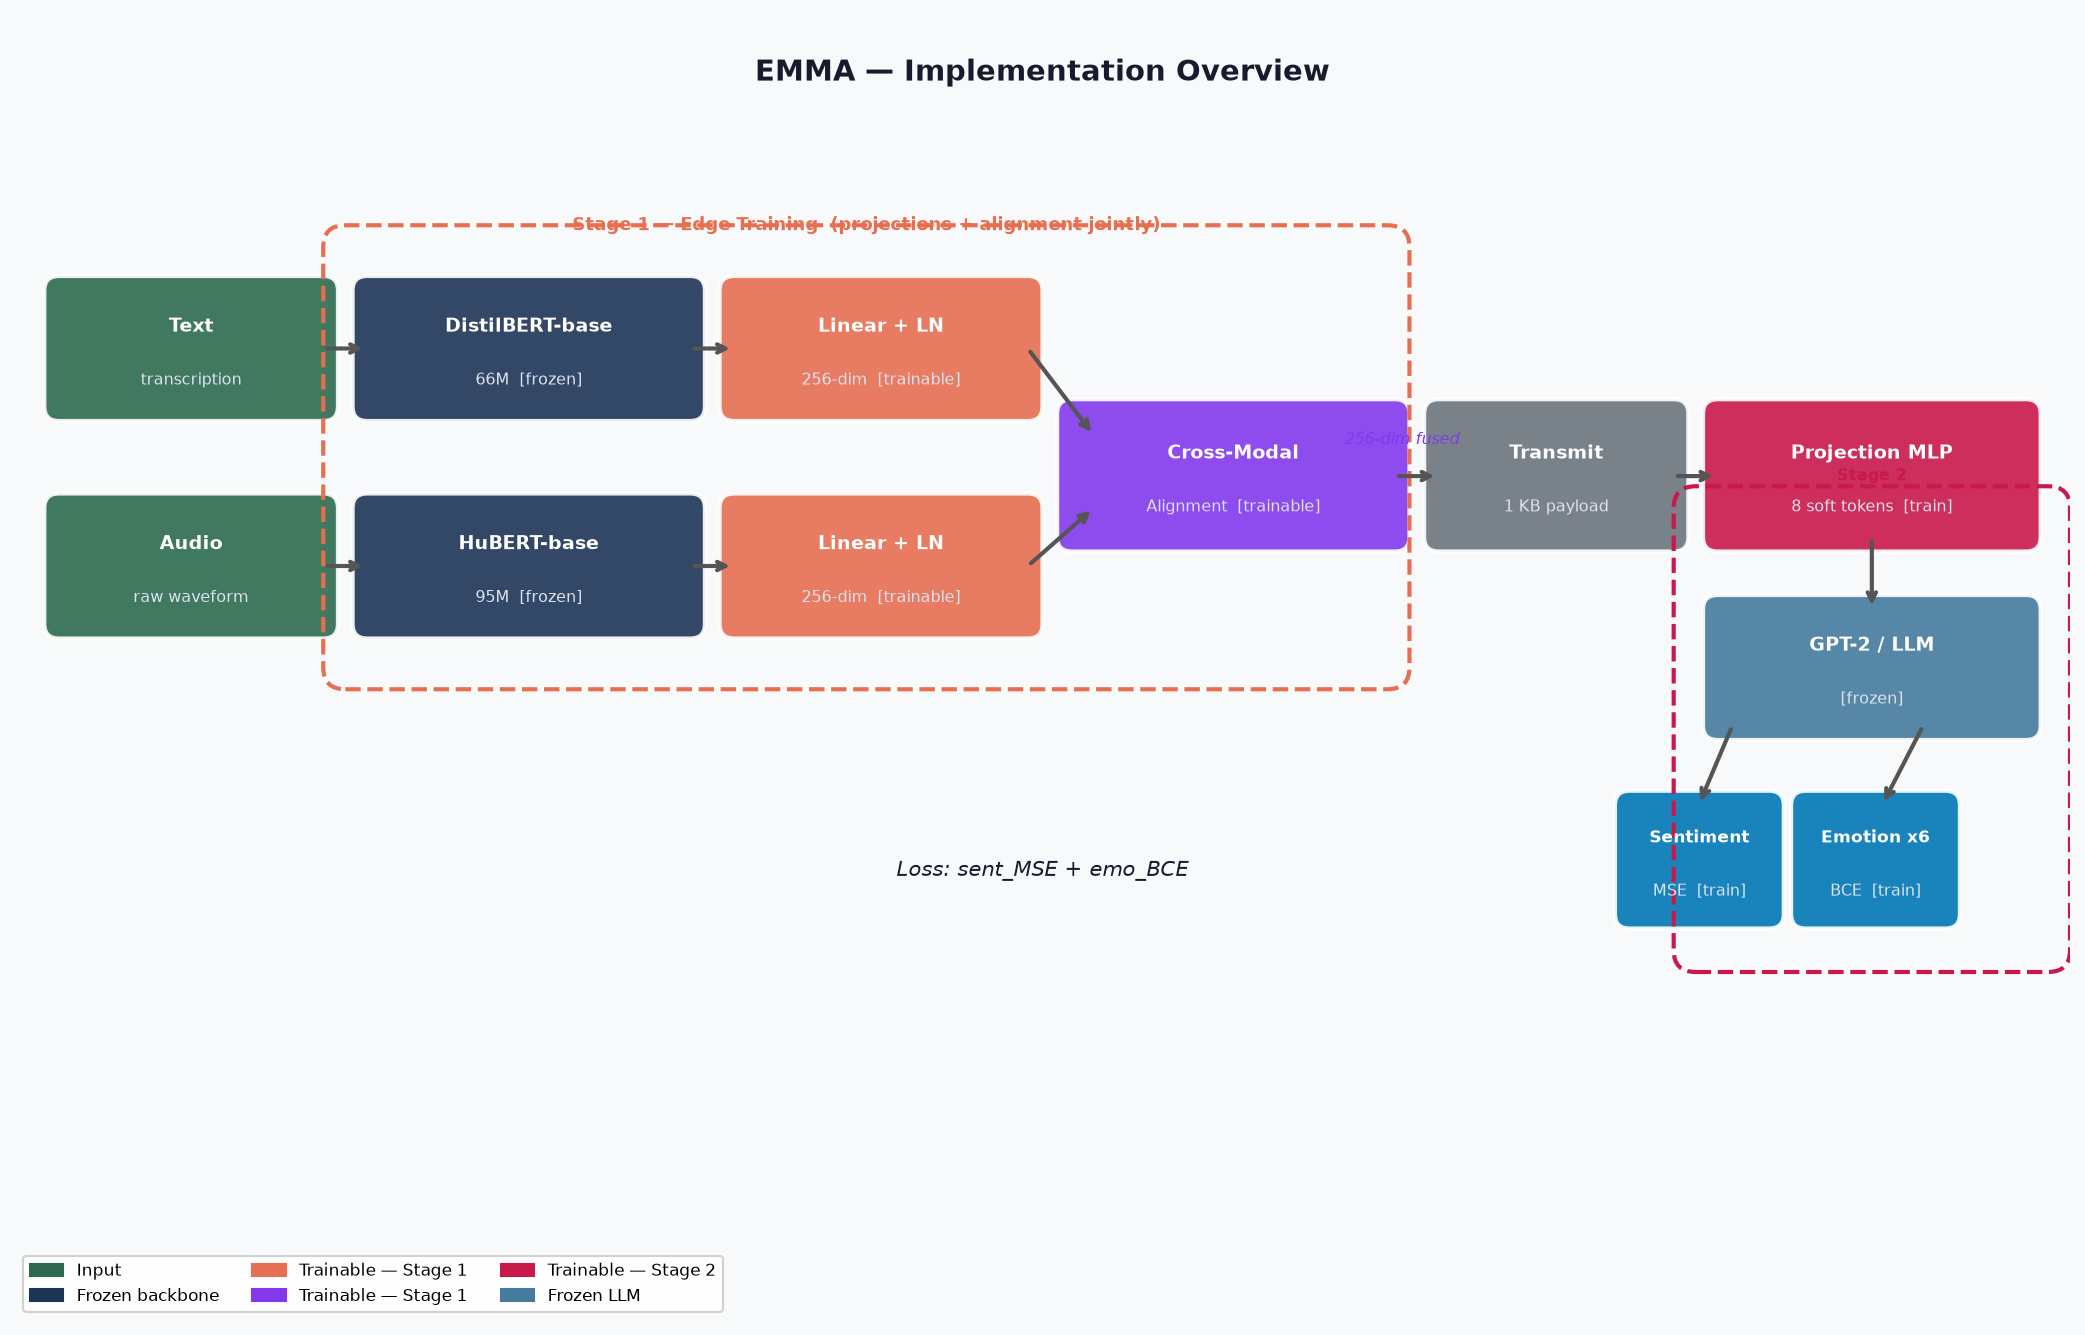
\includegraphics[width=\columnwidth]{emma_pipeline.png}
\caption{EMMI pipeline: encode, align, and compress at the edge;
decompress, project, and reason at the server.}
\label{fig:pipeline}
\end{figure}

\paragraph{Stage 1 — Encode.}
Each input modality passes through a frozen, pre-trained encoder that
maps raw input to a fixed-dimensional embedding. In our image-text
instantiation, an image encoder and a text encoder each produce a
512-dim vector. Encoders are frozen throughout: they do not participate
in training and can be replaced without modifying any other component.
This stage accounts for over 99\% of edge compute ($\sim$212\,ms);
every subsequent design choice is made under this constraint.

\paragraph{Stage 2 — Align.}
The per-modality embeddings $t, v \in \mathbb{R}^{512}$ are combined
into a single fused vector $f$ before compression. This step is where
cross-modal structure is made explicit: a good alignment operator gives
the compressor access to the \emph{relationship} between modalities,
not just the individual representations. As we show in
Section~\ref{sec:method}, this choice has a larger impact on downstream
accuracy than the choice of encoder or compression method.

\paragraph{Stage 3 — Compress.}
A lightweight encoder $g_\phi: \mathbb{R}^{d_f} \rightarrow \mathbb{R}^{64}$
maps the aligned representation to the transmitted latent
$z = g_\phi(f)$. Only $g_\phi$ runs on the edge; its counterpart
$g_\phi^{-1}$ (if used) resides on the server. The compression step adds
less than 0.65\,ms regardless of method --- it is effectively free
relative to encoding.

\subsection{Server Pipeline}

Upon receiving $z \in \mathbb{R}^{64}$, the server has no access to
the original images, text, or intermediate activations --- only the
compressed semantic summary produced by the edge.

\paragraph{Decompress.}
The received latent $z \in \mathbb{R}^{64}$ is passed through the
decoder $g_\phi^{-1}$, which reconstructs an approximation $\hat{f}$
of the original fused embedding. This recovers the full-dimensional
cross-modal representation before reasoning. We also evaluate projecting
directly from $z$ without decoding; the two variants perform
equivalently (Section~\ref{sec:eval}), indicating that the compressed
latent is itself sufficiently discriminative for the downstream task.

\paragraph{Project and reason.}
A learned MLP $p_\psi$ maps the decompressed representation to 8 soft
prompt tokens in the LLM's embedding space ($d_\text{LLM}{=}768$ for
GPT-2). These tokens are prepended to the LLM's context alongside a
natural-language instruction, and the LLM's final hidden state feeds a
binary classification head. The LLM is entirely frozen: it contributes
pre-trained language understanding without task-specific retraining and
can be replaced with a more capable model without modifying any edge
component. Only $p_\psi$ and the classification head are trained.

\subsection{Training Protocol and Decoupling}

EMMI is trained in two independent stages. First, the compressor
($g_\phi$, $g_\phi^{-1}$) is trained on the fused embeddings using
a compressor-specific loss (e.g., reconstruction for AE, contrastive
for ContrastiveAE, or variance maximization for PCA). Second, the
server projection $p_\psi$ is trained with the compressor frozen,
optimizing only the downstream task loss. No stage requires the other
to change.

This decoupling has a practical consequence: the edge compressor and the
server model can be deployed, updated, and versioned independently.
An edge device can compress with a fixed $g_\phi$ while the server
upgrades its LLM, and vice versa. In heterogeneous deployments where
edge and server are operated by different parties or on different update
cycles, this independence is not a convenience --- it is a requirement.


% ============================================================
\section{Proposed Method}
\label{sec:method}
% ============================================================

Two design choices in EMMI have disproportionate impact on accuracy:
how modalities are fused before compression, and how the fused
representation is compressed. This section motivates each choice and
explains why the standard alternatives fail.

\subsection{Match Fusion}

The simplest fusion operators --- mean and concatenation --- discard or
obscure the cross-modal relationship that is most informative for a
matching task. Mean fusion $(t + v)/2$ cancels the difference signal:
when $t \approx v$ (matched) and $t \not\approx v$ (non-matched), the
mean carries little discriminative information about \emph{how} the two
embeddings relate. Concatenation preserves both but does not expose
their relationship explicitly, leaving it to the compressor or server
to discover.

We instead use \textbf{match fusion}, which makes the relationship explicit:
\begin{equation}
f_\text{match} = \bigl[t;\;v;\;|t - v|;\;t \odot v\bigr] \in \mathbb{R}^{4d}
\label{eq:match}
\end{equation}
The four blocks serve distinct roles: $t$ and $v$ preserve the individual
modality signals; $|t-v|$ encodes \emph{disagreement} --- the
element-wise magnitude of mismatch between the two representations;
and $t \odot v$ encodes \emph{co-activation} --- dimensions where both
modalities respond strongly together. For a binary matching task, the
label is highly correlated with $\|t - v\|$, so making $|t-v|$ explicit
provides the compressor with a signal that is already partially aligned
with the supervision objective.

The cost is negligible: match fusion adds 0.013\,ms and expands the
vector from 512 to 2048 dimensions. The bandwidth cost is temporary ---
compression immediately reduces it back to 256 bytes regardless of
fusion mode.

\subsection{ContrastiveAE: Fixing the Compression Geometry}

\paragraph{Why standard compression fails for MobileCLIP.}
The root cause of compression failure is geometric. Standard methods
(PCA, AE, VAE) operate on the assumption that high-variance directions
in the embedding space carry the information worth preserving. For CLIP,
this assumption holds: CLIP's contrastive training objective explicitly
pulls matched pairs together and pushes non-matched pairs apart, so the
most variable dimensions in the embedding space are also the most
discriminative. PCA finds exactly these dimensions, which is why
CLIP compresses with near-zero accuracy loss.

MobileCLIP breaks this assumption. Its training objective does not
produce the same geometric alignment: task-discriminative information
is spread across low-variance directions that PCA and reconstruction-based
methods discard. The consequence is catastrophic --- PCA achieves only
57.4\% on match fusion (near-random), and plain AE achieves 53.2\%.
This is not a failure of the server or the fusion; it is a failure of
the compressed representation to carry the matching signal at all.

\paragraph{ContrastiveAE objective.}
The fix is to supervise the geometry of the compressed representation
directly. We train an autoencoder with a combined loss:
\begin{equation}
\mathcal{L} = \underbrace{\mathcal{L}_\text{MSE}(g_\phi^{-1}(z),\, f)}_{\text{reconstruct}}
            + \;\lambda \cdot \underbrace{\mathcal{L}_\text{SupCon}(\{z_i\}, \{y_i\})}_{\text{discriminate}}
\label{eq:cae}
\end{equation}
where $z_i = g_\phi(f_i)$ and $y_i \in \{0,1\}$ are binary match labels.
The Supervised Contrastive loss~\cite{khosla2020supcon} pulls latents
of matched pairs together and pushes non-matched pairs apart within the
64-dim bottleneck. Where reconstruction loss preserves the original
geometry (including its task-irrelevant high-variance structure),
the contrastive term \emph{reshapes} the geometry to be discriminative.

The result is a 64-dim space that is more task-aligned than the
original 512-dim embedding --- not despite compression, but because of it.
Labels are used only during compression training; at deployment the edge
runs $g_\phi$ alone, with no access to labels or the server.

\paragraph{Decode-on-server ablation.}
A natural question is whether the server should decode the latent before
projection. We tested this: decoding first achieves 98.25\% vs.\ 98.28\%
without decoding. The difference is within noise, confirming that the
64-dim latent is sufficiently discriminative for direct use and that
server-side decoding adds compute with no accuracy benefit.

\subsection{Unsupervised Alternatives}

ContrastiveAE requires binary labels during compression training.
For settings where these are unavailable, we evaluated several label-free
alternatives, which reveal a secondary insight: the \emph{structure of
match fusion} can be exploited even without supervision.

\textbf{BlockPCA} applies PCA independently to each of the four blocks
of $f_\text{match}$ --- 16 components per block, 64 total. Global PCA
on the 2048-dim vector discards the $|t{-}v|$ block because it is not the
highest-variance direction overall. BlockPCA preserves it because each
block is treated independently. The result is 97.80\% test accuracy
with no labels --- only 0.52pp below the uncompressed baseline and 0.48pp
below ContrastiveAE.

\textbf{CrossModalAE} uses the natural image-text pairing as free
supervision: an InfoNCE loss between the latent $z$ and the original
per-modality embeddings encourages $z$ to remain aligned with both
modalities without binary labels. It reaches 90--92\% across fusion
modes --- a substantial improvement over collapsed baselines, but below
ContrastiveAE.

\textbf{LDA} (Linear Discriminant Analysis) achieves 98.33\% on match
fusion with only a single discriminant dimension, confirming that the
matching signal is highly concentrated once the right geometric structure
is found. However, LDA requires binary labels at fitting time, making it
equivalent to ContrastiveAE in supervision requirements but less
flexible (no compression training, no neural encoder).


% ============================================================
\section{Evaluation}
\label{sec:eval}
% ============================================================

Having described the EMMI architecture and its two core contributions,
we now assess whether they deliver on the promises implied by the
system model: (i) that match fusion materially improves accuracy
over standard operators, (ii) that a lightweight encoder (MobileCLIP)
can outperform a heavier one (CLIP) when paired with the right fusion,
and (iii) that ContrastiveAE is the only compression method that
preserves accuracy under the 32$\times$ bandwidth constraint.

\subsection{Experimental Setup}

\paragraph{Task and dataset.}
Binary image-text matching on MS-COCO captions
(\texttt{clip-benchmark/wds\_mscoco\_captions}).
Splits: 72K train / 5K validation / 5K test. Validation accuracy
is used for model selection; test accuracy for final reporting.
All results are means over 3 seeds unless noted (5 seeds for CLIP
compression baselines).

\paragraph{Encoders.}
CLIP ViT-B/32: 87M image-encoder parameters, 512-dim output.
MobileCLIP2-S0: 11.4M image-encoder parameters, 512-dim output
(without L2 normalization).

\paragraph{Server.}
Frozen GPT-2 (117M parameters, 768-dim) with 8 learned soft-prompt
tokens and a binary classification head. Only the projection MLP
($\sim$100K parameters) and head are trained.

\paragraph{Compression target.}
All methods compress to $k{=}64$ dimensions (256 bytes).

\subsection{Fusion Mode Ablation}

Table~\ref{tab:fusion} tests whether match fusion's design advantage
translates into measured accuracy. It does --- consistently, across both
encoders. More strikingly, the accuracy gap between encoders reverses
under match fusion: MobileCLIP underperforms CLIP by 1.3pp under mean
fusion but \emph{outperforms} it by 0.34pp under match fusion.
Match fusion does not merely improve accuracy; it changes which encoder
is the better choice.

\begin{table}[h]
\centering
\caption{Accuracy (\%) by encoder and fusion. No compression. 3 seeds.}
\label{tab:fusion}
\begin{tabular}{llcc}
\toprule
Encoder & Fusion & Val (\%) & Test (\%) \\
\midrule
CLIP ViT-B/32   & mean   & 94.45 & 94.19 \\
CLIP ViT-B/32   & concat & 96.77 & 96.87 \\
CLIP ViT-B/32   & match  & 97.99 & 97.98 \\
\midrule
MobileCLIP2-S0  & mean   & 93.10 & 92.79 \\
MobileCLIP2-S0  & concat & 95.96 & 96.05 \\
MobileCLIP2-S0  & match  & \textbf{98.51} & \textbf{98.32} \\
\bottomrule
\end{tabular}
\end{table}

\subsection{Compression: CLIP}

For CLIP, the compression question is straightforward. Table~\ref{tab:clip_compression}
shows that all four standard methods preserve accuracy within 0.5pp ---
in fact, all four \emph{improve} slightly on the uncompressed baseline,
suggesting mild regularization from the bottleneck. This is the expected
behaviour when the embedding geometry is task-aligned.

\begin{table}[h]
\centering
\caption{CLIP + mean fusion, 64-dim compression. 5 seeds each.}
\label{tab:clip_compression}
\begin{tabular}{lccc}
\toprule
Method & Val (\%) & Test (\%) & $\Delta$ Test \\
\midrule
None (512-dim)  & 94.45 & 94.19 & --- \\
PCA             & 94.65 & 94.48 & $+$0.29 \\
AE              & 94.43 & 94.32 & $+$0.13 \\
VAE             & 94.38 & 94.23 & $+$0.04 \\
DistilAE        & 94.79 & 94.60 & $+$0.41 \\
\bottomrule
\end{tabular}
\end{table}

\subsection{Compression: MobileCLIP}

The MobileCLIP results in Table~\ref{tab:mc_compression} tell a different
story. Every standard method collapses on at least one fusion mode ---
PCA, AE, VAE, DistilAE, and LDA all drop to near-random accuracy ($\sim$50\%)
on concat fusion, and most collapse on match fusion too. This is not
overfitting or a hyperparameter issue: the collapse is systematic, stable
across seeds, and present regardless of compression architecture. The
geometric mismatch described in Section~\ref{sec:method} is real and severe.

ContrastiveAE is the only method that does not collapse on any fusion mode.
More than that: it achieves \emph{higher} accuracy than the uncompressed
baseline on mean ($+$0.39pp) and concat ($+$0.83pp) fusions, because the
contrastive term reshapes the embedding geometry to be more task-aligned
than the original. On match fusion --- where the structure already
partially exposes the matching signal --- it preserves 98.28\% test
accuracy, within noise of the uncompressed 98.32\%.

\paragraph{Decode-on-server ablation.}
Table~\ref{tab:mc_compression} also reports ContrastiveAE+decode, where
the server reconstructs $\hat{f} = g_\phi^{-1}(z)$ before projection.
Direct projection from $z$ outperforms decoding first (98.28\% vs.\
98.25\%), suggesting the 64-dim latent is information-sufficient for
this task. This result should not be generalized, however. Compression
is lossy by construction, and ContrastiveAE is trained to preserve the
\emph{matching} signal specifically. For tasks requiring richer
cross-modal reasoning --- visual question answering, caption generation,
or multi-label classification --- the mutual information between the
latent and the task label, $I(z;\,y)$, may fall below $I(f;\,y)$,
meaning the bottleneck discards signal the server needs. In such
settings, server-side decoding recovers an approximation of the
full-dimensional representation, which may improve task accuracy at
the cost of an additional decoder forward pass. The optimal
configuration --- decode or project directly --- should therefore be
treated as task-dependent, determined by whether the compression
bottleneck is information-sufficient for the target task.

\begin{table}[h]
\centering
\caption{MobileCLIP compression to 64-dim. 3 seeds unless noted
($\dag$: 1 seed). *Near-random; compression collapsed.}
\label{tab:mc_compression}
\begin{tabular}{llccc}
\toprule
Fusion & Method & Val (\%) & Test (\%) & $\Delta$ Test \\
\midrule
mean  & None            & 93.10 & 92.79 & --- \\
mean  & PCA$^\dag$      & 80.54 & 80.01 & $-$12.8 \\
mean  & AE              & 79.24 & 79.04 & $-$13.8 \\
mean  & VAE$^\dag$      & 77.53 & 76.58 & $-$16.2 \\
mean  & DistilAE$^\dag$ & 70.29 & 70.47 & $-$22.3 \\
mean  & LDA$^\dag$      & 80.75 & 80.65 & $-$12.1 \\
mean  & CrossModalAE$^\dag$ & 91.90 & 92.06 & $-$0.73 \\
mean  & \textbf{ContrastiveAE} & \textbf{93.49} & \textbf{93.18} & \textbf{$+$0.39} \\
\midrule
match & None            & 98.51 & 98.32 & --- \\
match & AE              & 52.97 & 53.17 & $-$45.2* \\
match & VAE$^\dag$      & 69.48 & 69.87 & $-$28.5 \\
match & DistilAE$^\dag$ & 82.90 & 83.06 & $-$15.3 \\
match & PCA$^\dag$      & 56.95 & 57.35 & $-$41.0* \\
match & CrossModalAE$^\dag$ & 90.79 & 90.30 & $-$8.0 \\
match & LDA$^\dag$      & 98.21 & 98.33 & $+$0.01 \\
match & BlockPCA        & 98.02 & 97.80 & $-$0.52 \\
match & \textbf{ContrastiveAE} & \textbf{98.62} & \textbf{98.28} & \textbf{$-$0.04} \\
match & ContrastiveAE+decode$^\dag$ & 98.42 & 98.25 & $-$0.07 \\
\midrule
concat & None           & 95.96 & 96.05 & --- \\
concat & AE             & 50.29 & 50.33 & $-$45.7* \\
concat & VAE$^\dag$     & 50.10 & 50.03 & $-$46.0* \\
concat & DistilAE$^\dag$& 50.60 & 50.52 & $-$45.5* \\
concat & PCA$^\dag$     & 50.12 & 50.08 & $-$46.0* \\
concat & LDA$^\dag$     & 50.00 & 49.96 & $-$46.1* \\
concat & CrossModalAE$^\dag$ & 90.79 & 90.51 & $-$5.5 \\
concat & \textbf{ContrastiveAE} & \textbf{96.81} & \textbf{96.88} & \textbf{$+$0.83} \\
\bottomrule
\end{tabular}
\end{table}

\subsection{Pipeline Latency}

Accuracy is necessary but not sufficient for edge deployment. We now ask:
does the EMMI pipeline meet the latency requirements of a constrained
edge device, and where does compression actually help?

Timings are wall-clock on a single CPU thread (200 runs, 30 warm-up) on
an Intel x86\_64 compute node. Single-thread CPU provides a reproducible
worst-case proxy for constrained edge hardware.

\begin{table}[h]
\centering
\caption{Edge-side latency: single CPU thread, mean $\pm$ std (ms).}
\label{tab:latency_edge}
\begin{tabular}{lcc}
\toprule
Component & CLIP ViT-B/32 & MobileCLIP2-S0 \\
\midrule
Image encoder     & $133.0 \pm 4.7$  & $139.1 \pm 1.5$ \\
Text encoder      & $81.2  \pm 1.8$  & $74.6  \pm 3.1$ \\
Both encoders     & $215.3 \pm 6.6$  & $\mathbf{212.4 \pm 3.4}$ \\
\midrule
Match fusion (2048-dim)           & \multicolumn{2}{c}{$0.013 \pm 0.000$} \\
PCA-64 encoder (2048$\to$64)      & \multicolumn{2}{c}{$0.011 \pm 0.001$} \\
BlockPCA-64 encoder               & \multicolumn{2}{c}{$0.014 \pm 0.001$} \\
AE-64 / ContrastiveAE-64 encoder  & \multicolumn{2}{c}{$0.641 \pm 0.005$} \\
\midrule
Server: GPT-2 inference           & \multicolumn{2}{c}{$156.2 \pm 3.0$} \\
\bottomrule
\end{tabular}
\end{table}

Two latency findings stand out. First, MobileCLIP and CLIP have nearly
identical total encoder latency (212 vs.\ 215\,ms), but MobileCLIP is
$1.9\times$ more consistent (3.4 vs.\ 6.6\,ms std). For real-time systems
with latency budgets, predictability matters as much as mean latency.
Second, all post-encoding steps --- fusion and compression --- add less than
1\,ms combined. The encoder accounts for over 99\% of edge compute
regardless of which compression method is chosen.

This means the compression choice has no meaningful impact on edge
compute latency. Its impact is entirely on the network:

\begin{table}[h]
\centering
\caption{Transmission latency (ms) $=$ payload $\div$ bandwidth. Mathematical.}
\label{tab:latency_tx}
\begin{tabular}{lcccc}
\toprule
Payload & IoT & LTE & WiFi & 5G \\
        & 0.1\,Mbps & 10\,Mbps & 50\,Mbps & 100\,Mbps \\
\midrule
Match, uncompressed (8\,192\,B)  & 655.4 & 6.6 & 1.3 & 0.7 \\
Concat, uncompressed (4\,096\,B) & 327.7 & 3.3 & 0.7 & 0.3 \\
Mean, uncompressed (2\,048\,B)   & 163.8 & 1.6 & 0.3 & 0.2 \\
\textbf{Compressed, 64-dim (256\,B)} & \textbf{20.5} & \textbf{0.2} & \textbf{0.04} & \textbf{0.02} \\
\bottomrule
\end{tabular}
\end{table}

On IoT links (0.1\,Mbps) --- the regime where EMMI is most needed ---
compression reduces transmission from 655\,ms to 20\,ms, a saving of
635\,ms per query. Combined with the server inference time of 156\,ms,
the full round-trip drops from $\sim$1024\,ms to $\sim$389\,ms: a
\textbf{2.6$\times$ end-to-end speedup} with no accuracy cost.
On WiFi/5G, transmission is negligible ($<$2\,ms) and the choice of
compression method makes no latency difference --- only accuracy matters,
which again favours ContrastiveAE.


% ============================================================
\section{Conclusion}
\label{sec:conclusion}
% ============================================================

We presented EMMI, an edge-server multimodal inference system that achieves
high accuracy under strict bandwidth constraints. The experiments surface
three findings, each with implications beyond this specific evaluation.

\textbf{Fusion operators are not interchangeable.} Match fusion
outperforms mean and concat fusion by up to 5.5\,pp and reverses the
accuracy ranking between encoders. Its explicit difference and
co-activation signals are particularly important for compressed
representations, where the server has less information to work with.

\textbf{Lightweight encoders can dominate with the right fusion.}
MobileCLIP2-S0 (11.4M parameters) achieves 98.32\% test accuracy
vs.\ CLIP's 97.98\%, with $1.9\times$ more consistent latency. Under
mean or concat fusion it underperforms CLIP; under match fusion it
surpasses it. Encoder choice and fusion choice must be made jointly.

\textbf{Compression geometry is encoder-specific and must be supervised.}
Standard compression methods that succeed for CLIP collapse catastrophically
for MobileCLIP. ContrastiveAE resolves this by directly supervising the
bottleneck geometry, achieving 98.28\% test with a 32$\times$ bandwidth
reduction and a 2.6$\times$ end-to-end speedup on IoT links.

While this paper evaluates EMMI on image-text matching as an initial
instantiation, the architecture is modality-agnostic. The edge pipeline
generalizes to any combination of inputs --- audio, telemetry, GPS,
sensor streams --- by replacing the per-modality encoders; match fusion
and ContrastiveAE operate on the fused embedding without
modality-specific modifications. Extending EMMI to the richer sensor
combinations found in autonomous edge systems, such as drone perception
with visual, acoustic, and GPS streams, is a direct avenue for future work.

\bibliographystyle{IEEEtran}
\bibliography{references}

\end{document}
